\documentclass[tikz]{standalone}
\usepackage{frenchmath}

\begin{document}
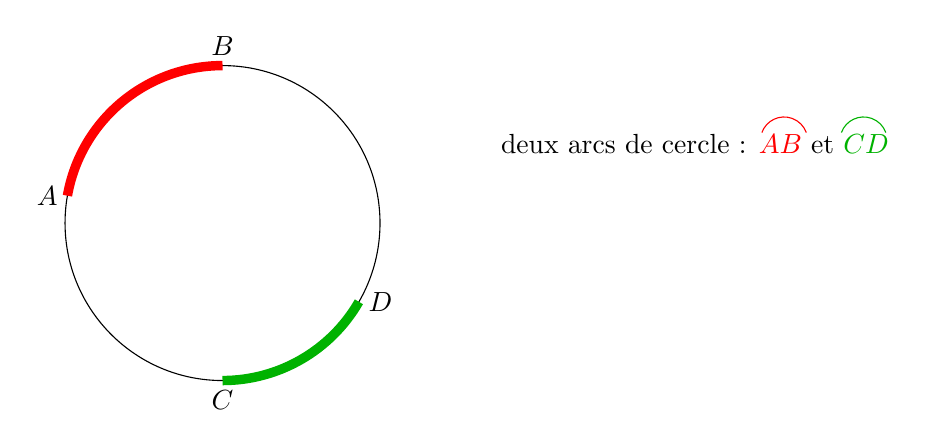
\begin{tikzpicture}
    \draw (0,0) circle (2);
    \coordinate (A) at ({2*cos(170)},{2*sin(170});
    \coordinate (B) at ({2*cos(90)},{2*sin(90});
    \coordinate (C) at ({2*cos(270)},{2*sin(270});
    \coordinate (D) at ({2*cos(330)},{2*sin(330});
    \draw[line width=1.2mm,red] (A) arc (170:90:2);
    \draw[line width=1.2mm,green!70!black] (C) arc (270:330:2);
    \foreach \p/\x in {A/left,B/above,C/below,D/right} {
        \node[\x] at (\p) {$\p$};
    }
    \draw[red] (6.85,1.15) arc (160:20:0.3);
    \draw[green!70!black] (7.86,1.15) arc (160:20:0.3);
    \node at (6,1) {deux arcs de cercle : \textcolor{red}{$AB$} et \textcolor{green!70!black}{$CD$}};
\end{tikzpicture}
\end{document}